El reto consiste en diseñar un procedimiento para escribir/leer un árbol binario a/de disco de forma que se recupere la estructura jerárquica de forma unívoca usando el mínimo número de centinelas que veáis posible. El reto queda resuelto simplemente rebajando el número de centinelas que se usaron en clase cuando se comentó el método de lectura/escritura preorden con centinelas.\\


    En clase, se vio que para cada nodo donde podría ir un nodo pero no iba, se colocaba un centinela, $-1$. De esta forma, los nodos hoja iban seguidos de dos $-1$, ya que debían especificar que no tenían ni hijo izquierda ni hijo derecha. Veamos un ejemplo:
    \begin{figure}[H]
        \centering
        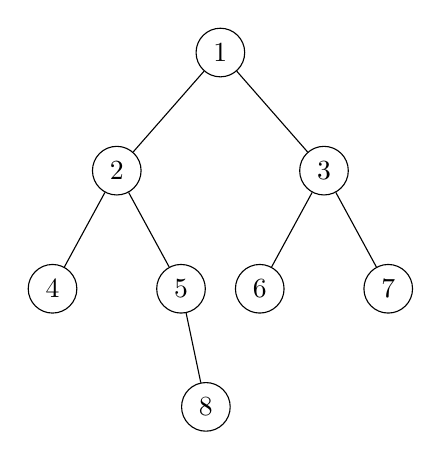
\begin{tikzpicture}[
            every node/.style={circle, draw},
            level 1/.style={sibling distance=2cm},
            level 2/.style={sibling distance=1cm},
            level 3/.style={sibling distance=1cm},
            level distance=1.5cm,
            ]
            \node {1}
            child[left] {node {2}
              child[left] {node {4}}
              child[right] {node {5}
                child[right] {node {8}} 
              }
            }
            child[right] {node {3}
              child[left] {node {6}}
              child[right] {node {7}}
            };
            \end{tikzpicture}
        \caption{Árbol binario que no está completo.}
        \label{fig:arb_1}
    \end{figure}

    Según la forma vista en clase, la forma de determinar dicho árbol sería:
    \begin{equation*}
        1~2~4~\red{\mathbf{-1}}~\red{\mathbf{-1}}~5~\red{\mathbf{-1}}~8~\red{\mathbf{-1}}~\red{\mathbf{-1}}~3~6~\red{\mathbf{-1}}~\red{\mathbf{-1}}~7~\red{\mathbf{-1}}~\red{\mathbf{-1}}
    \end{equation*}
    
    
    
    
    Una primera mejora es usar, para los nodos hoja, el centinela $-2$. De esta forma, no es necesario guardar dos centinelas, sino uno; ahorrándonos así un gran número de centinelas. Veamos un ejemplo:
    

    Tenemos que el árbol de la Figura \ref{fig:arb_1} queda únicamente determinado por el siguiente listado en preorden usando los centinela $-2$ para los nodos hoja y $-1$ para los nodos que, sin ser hoja, no están completos:
    \begin{equation*}
        1~2~4~\red{\mathbf{-2}}~5~\red{\mathbf{-1}}~8~\red{\mathbf{-2}}~3~6~\red{\mathbf{-2}}~7~\red{\mathbf{-2}}
    \end{equation*}

    Además, el último nodo (que siempre será una hoja) tampoco necesita de centinela, por lo que el último $-2$ no es necesario:
    \begin{equation*}
        1~2~4~\red{\mathbf{-2}}~5~\red{\mathbf{-1}}~8~\red{\mathbf{-2}}~3~6~\red{\mathbf{-2}}~7
    \end{equation*}

    De esta forma, si el número de nodos hoja es $H$ y en total se usaban $C$ centinelas de la primera, ahora se usarán:
    \begin{equation*}
        C'=C-H-1
    \end{equation*}
    Esto se debe a que cada nodo hoja usa un centinela en vez de dos, y el $-1$ se debe a que el último nodo hoja no usa ningún centinela.